\section{Interfejs graficzny}
\subsection{Ogólny diagram przejść}
\begin{figure}[h]
\begin{center}
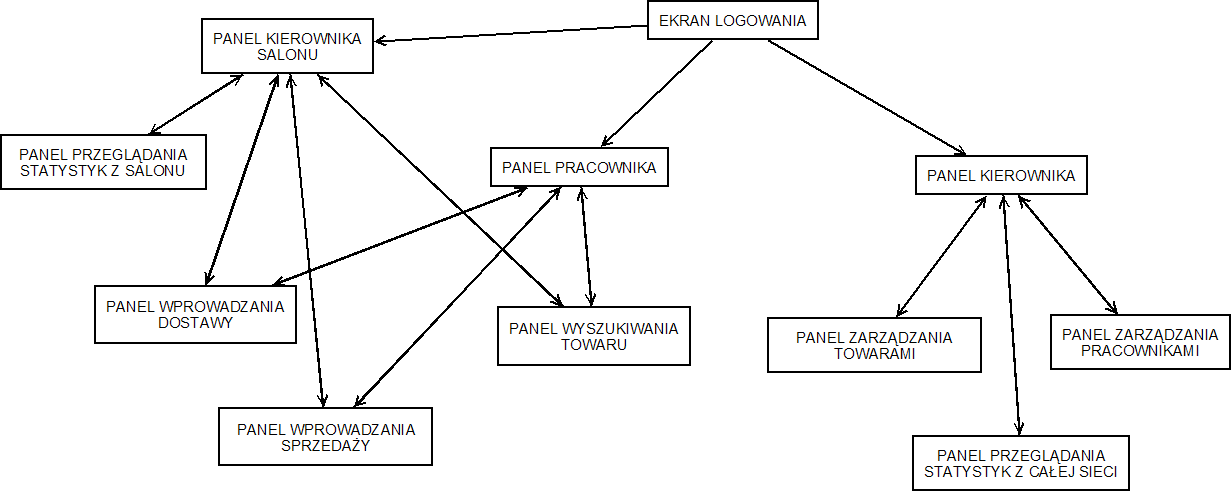
\includegraphics[width=1\textwidth]{gfx/diagram_przejsc.png}
\caption{Ogólny diagram przejść dla interfejsu graficznego}
\end{center}
\end{figure}
Na~tym ani kolejnych diagramach przejść, ze~względu na~chęć utrzymania przejrzystości, nie~został uwzględniony panel pomocy.

Do~panelu pomocy powinny ze~wszystkich paneli być poprowadzone strzałki "Kliknięcie <<Pomoc>>", a~z~niego do~wszystkich paneli powinny być poprowadzone strzałki "Kliknięcie <<Zamknij>>".
\clearpage
\subsection{Okno logowania}
\begin{figure}[h]
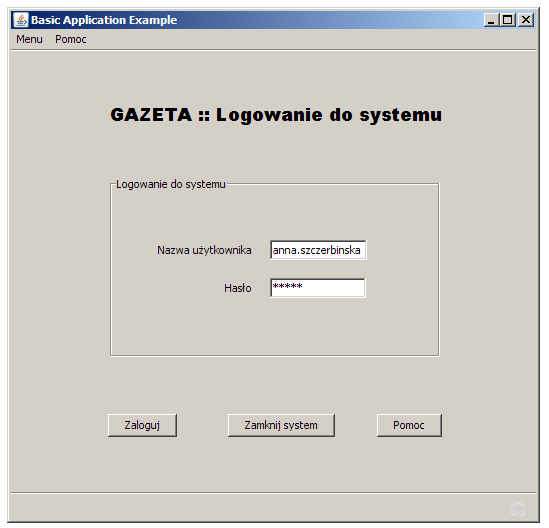
\includegraphics[width=1\textwidth]{gfx/logowanie.png}
\caption{Widok okna logowania do~systemu}
\end{figure}
\clearpage
\subsection{Panel pracownika}
\subsubsection{Diagram przejść dla panelu pracownika}
\begin{figure}[h]
\begin{center}
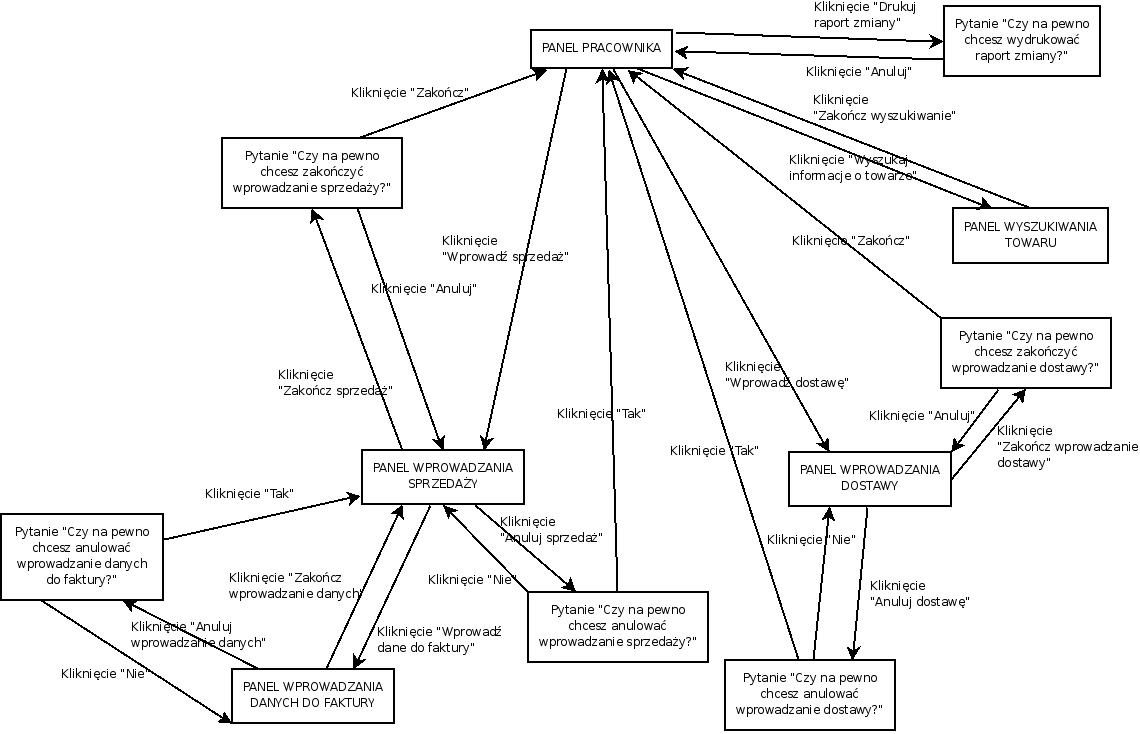
\includegraphics[width=15cm,angle=90,keepaspectratio]{gfx/przejscia_pracownik.png}
\caption{Diagram przejść dla panelu pracownika}
\end{center}
\end{figure}
\clearpage
\subsubsection{Panel pracownika}
\begin{figure}[h]
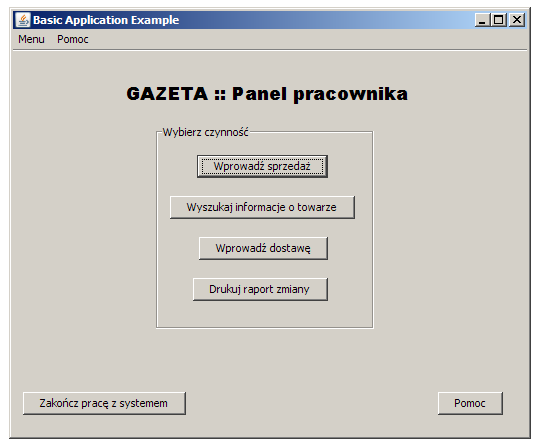
\includegraphics[width=1\textwidth]{gfx/pracownik.png}
\caption{Widok panelu pracownika}
\end{figure}
Wybór opcji "Wprowadź sprzedaż", "Wyszukaj informacje o towarze" lub "Wprowadź dostawę" powoduje otwarcie nowego okna z~odpowiednim panelem.

Wybór opcji "Drukuj raport zmiany" powoduje automatyczne wygenerowanie i~wydrukowanie raportu zmiany.
\clearpage
\subsubsection{Panel wprowadzania sprzedaży}
\begin{figure}[h]
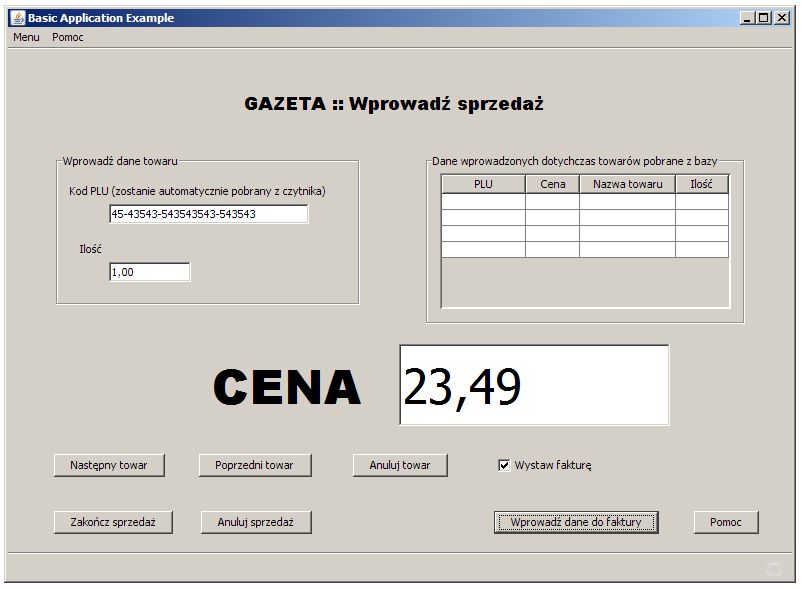
\includegraphics[height=1\textwidth,angle=90,keepaspectratio]{gfx/sprzedaz.png}
\caption{Widok panelu wprowadzania sprzedaży}
\end{figure}
W tabelce znajdują~się dane wczytanych w~ramach tej sprzedaży towarów. W~ramce "CENA" znajduje~się sumaryczna wartość towarów umieszczonych w~tabelce.

Po~wczytaniu czytnikiem lub~ręcznym wprowadzeniu kodu PLU i~ewentualnej zmianie ilości towaru (z~domyślnej 1,00 na~inną) dane towaru zostaną dodane do~tabelki (jako~kolejny wiersz).

Aby~zatwierdzić bieżący i~wprowadzić kolejny towar, należy wybrać opcję "Następny towar". Aby~edytować poprzednio wprowadzony towar, należy wybrać opcję "Poprzedni towar". Aby~anulować wprowadzanie towaru lub~usunąć~go z~listy sprzedaży, należy wybrać opcję "Anuluj towar". Aby~anulować wprowadzanie sprzedaży, należy wybrać opcję "Anuluj sprzedaż". Aby~zakończyć wprowadzanie sprzedaży, należy wybrać opcję "Zakończ sprzedaż".

Aby~edytować aktualnie wprowadzany towar, należy ponownie wprowadzić kod PLU lub~ilość (wtedy dane w~tabelce zostaną automatycznie uaktualnione).

Aby~wystawić fakturę za~wprowadzaną transakcję, należy zaznaczyć pole "Wystaw fakturę", a~następnie wybrać opcję "Wprowadź dane do~faktury". W~nowym oknie zostanie otwarty panel wprowadzania danych do~faktury.
\clearpage
\subsubsection{Panel wyszukiwania towaru}
\begin{figure}[h]
\begin{center}
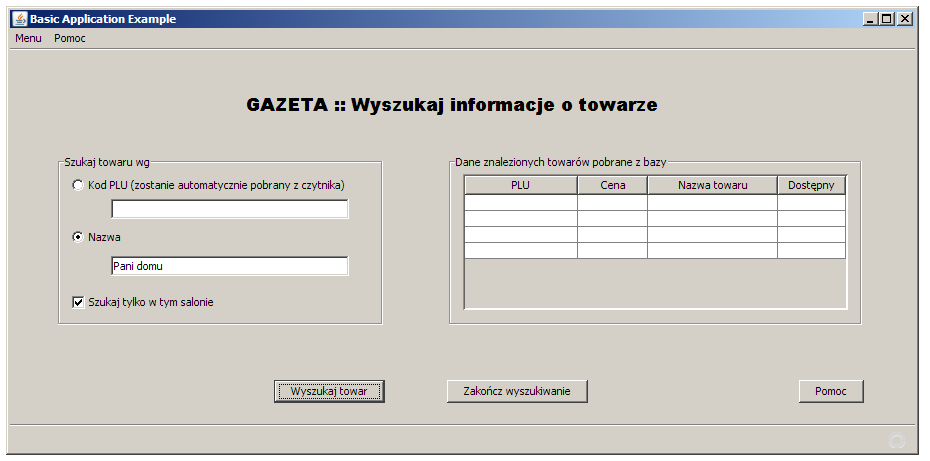
\includegraphics[width=20cm,angle=90,keepaspectratio]{gfx/wyszukaj_produkt.png}
\end{center}
\caption{Widok panelu wyszukiwania towaru}
\end{figure}
W tabelce znajdują~się dane znalezionych przez~wyszukiwarkę towarów.

Po wczytaniu czytnikiem lub~ręcznym wprowadzeniu kodu PLU lub~nazwy towaru i~wybraniu opcji "Wyszukaj towar" dane towarów pasujących do~opisu zostaną umieszczone w~tabelce.
W zależności od~tego, czy~szukamy towarów dostępnych tylko w~tym salonie, czy~w~całej sieci, można zaznaczyć lub~nie pole "Szukaj tylko w~tym salonie".
\clearpage
\subsubsection{Panel wprowadzania dostawy}
\begin{figure}[h]
\begin{center}
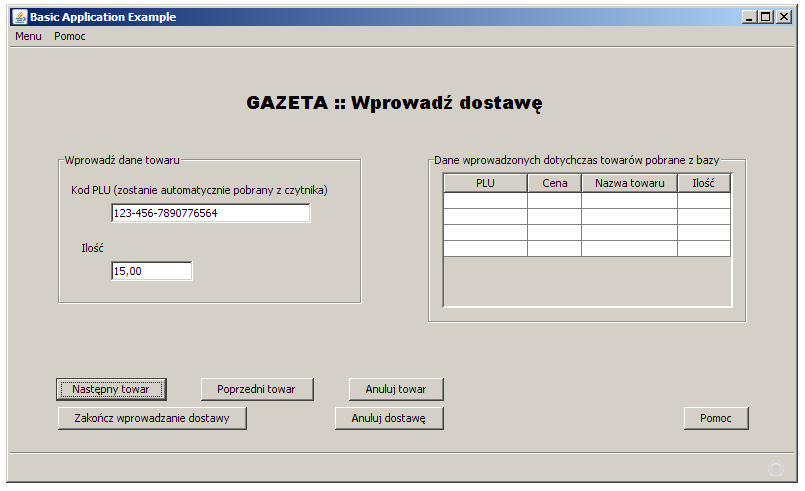
\includegraphics[width=20cm,angle=90,keepaspectratio]{gfx/dostawa.png}
\end{center}
\caption{Widok panelu wprowadzania dostawy}
\end{figure}
W~tabelce znajdują~się dane wczytanych w~ramach tej~dostawy towarów.

Po~czytaniu czytnikiem lub~ręcznym wprowadzeniu kodu PLU i~ewentualnej zmianie ilości towaru (z~domyślnej 1,00 na~inną) dane towaru zostaną dodane do~tabelki (jako~kolejny wiersz).

Aby~zatwierdzić bieżący i~wprowadzić kolejny towar, należy wybrać opcję "Następny towar". Aby~edytować poprzednio wprowadzony towar, należy wybrać opcję "Poprzedni towar". Aby~anulować wprowadzanie towaru lub~usunąć~go z~listy dostawy, należy wybrać opcję "Anuluj towar". Aby~anulować wprowadzanie dostawy, należy wybrać opcję "Anuluj dostawę". Aby~zakończyć wprowadzanie dostawy, należy wybrać opcję "Zakończ wprowadzanie dostawy".
Edytować aktualnie wprowadzany towar można na~dwa sposoby - albo~ponownie wprowadzić kod PLU lub~ilość (wtedy dane w~tabelce zostaną automatycznie uaktualnione), albo~kliknąć na~odpowiednie pole w~tabelce i~wprowadzić do~niej nową nazwę lub~cenę towaru.
\clearpage
\subsubsection{Panel wprowadzania danych do faktury}
\begin{figure}[h]
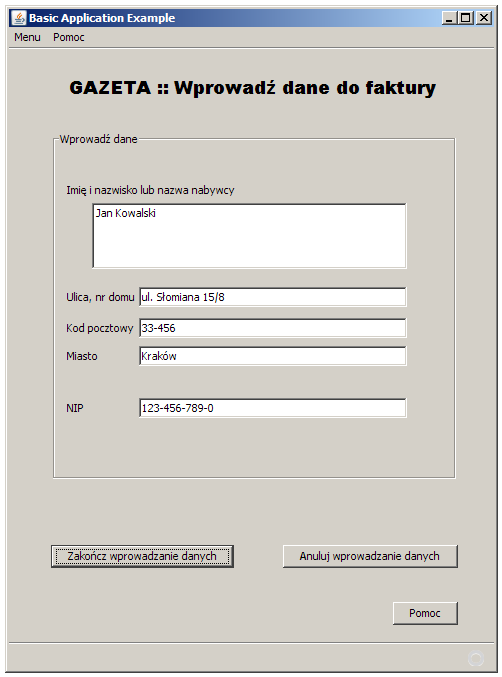
\includegraphics[width=1\textwidth]{gfx/dane_faktury.png}
\caption{Widok panelu wprowadzania danych do faktury}
\end{figure}
Po wypełnieniu formularza danymi klienta należy wybrać opcję "Zakończ wprowadzanie danych", aby~zatwierdzić dane, albo "Anuluj wprowadzanie danych", aby~zrezygnować z~ich wprowadzania do~faktury. Po~wybraniu dowolnej z~tych opcji następuje zamknięcie panelu wprowadzania danych do~faktury i~powrót do~panelu wprowadzania sprzedaży (który nie został zamknięty w~chwili wyboru opcji wprowadzenia danych do~faktury).
\clearpage
\subsection{Panel kierownika salonu}
\subsubsection{Diagram przejść dla panelu kierownika salonu}
\begin{figure}[h]
\begin{center}
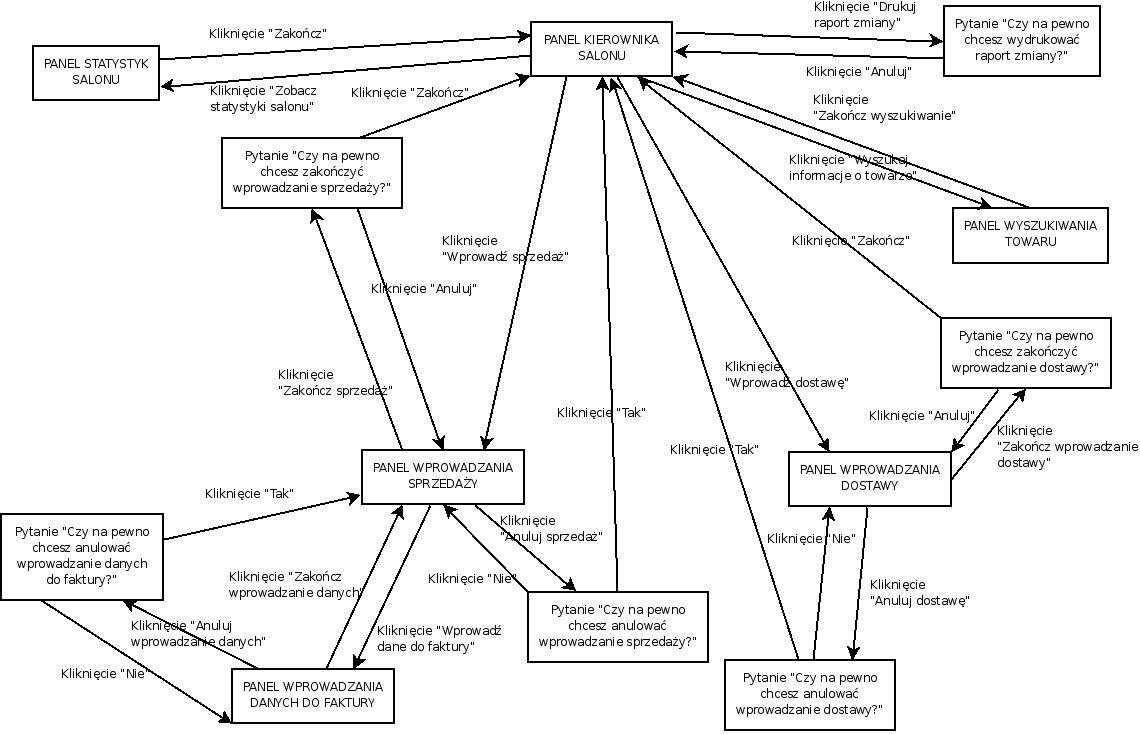
\includegraphics[width=15cm,angle=90,keepaspectratio]{gfx/przejscia_kierownik.png}
\caption{Diagram przejść dla panelu kierownika salonu}
\end{center}
\end{figure}
\clearpage
\subsubsection{Panel kierownika salonu}
\begin{figure}[h]
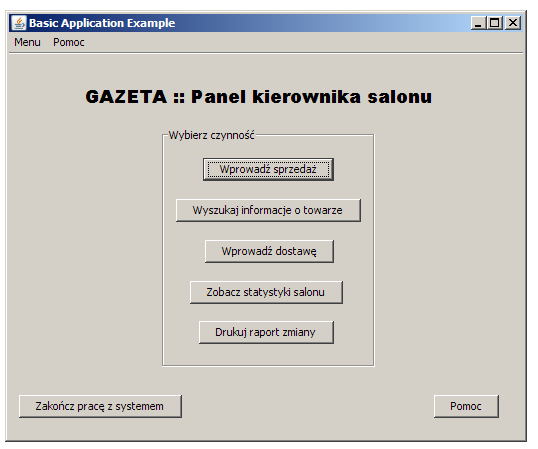
\includegraphics[width=1\textwidth]{gfx/kierownik.png}
\caption{Widok panelu kierownika salonu}
\end{figure}
Wybór opcji "Wprowadź sprzedaż", "Wyszukaj informacje o towarze" lub "Wprowadź dostawę" powoduje otwarcie nowego okna z~odpowiednim panelem (tego samego, co w~przypadku panelu pracownika).

Wybór opcji "Zobacz statystyki salonu" powoduje otwarcie nowego okna z~panelem statystyk salonu.

Wybór opcji "Drukuj raport zmiany" powoduje automatyczne wygenerowanie i~wydrukowanie raportu zmiany.
\clearpage
\subsubsection{Panel statystyk salonu}
\begin{figure}[h]
\begin{center}
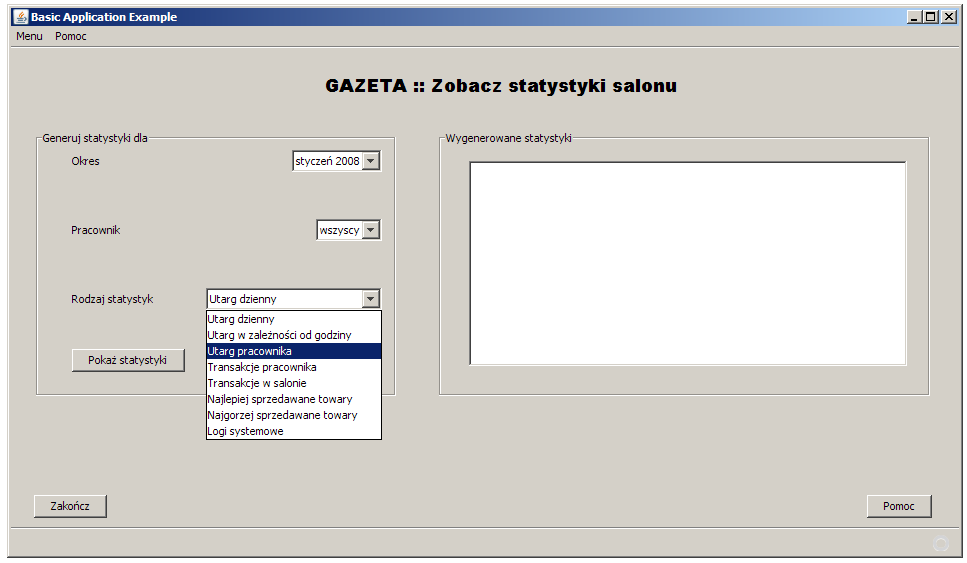
\includegraphics[width=20cm,angle=90,keepaspectratio]{gfx/stat_salonu.png}
\end{center}
\caption{Widok panelu statystyk salonu}
\end{figure}
W formularzu należy wybrać okres, za~który mają zostać wygenerowane statystyki, pracowników, których statystyki mają dotyczyć, oraz~rodzaj statystyk. Wybór opcji "Pokaż statystyki" powoduje wygenerowanie (na podstawie danych pobranych w~tym celu z~bazy) statystyk odpowiadających danym z~formularza i~wyświetlenie ich w~formie graficznej (lub tekstowej, w~przypadku logów systemowych) w~ramce "Wygenerowane statystyki".

Aby~zakończyć oglądanie statystyk salonu i~powrócić do~panelu kierownika salonu, należy wybrać opcję "Zakończ".
\clearpage
\subsection{Panel kierownika}
\subsubsection{Diagram przejść dla panelu kierownika}
\begin{figure}[h]
\begin{center}
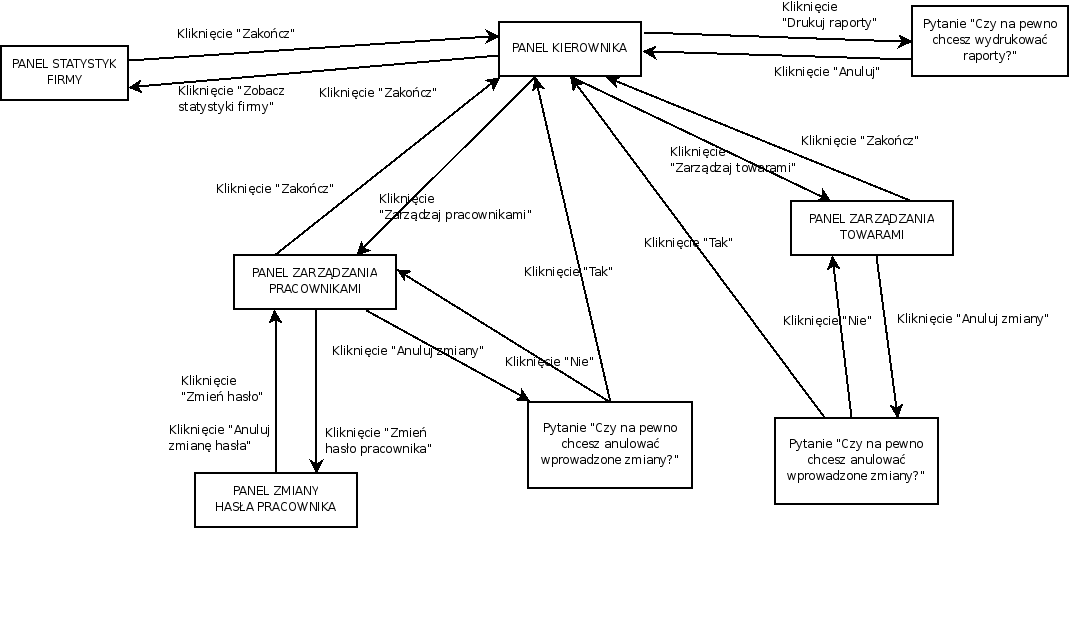
\includegraphics[width=15cm,angle=90,keepaspectratio]{gfx/przejscia_szef.png}
\caption{Diagram przejść dla panelu kierownika}
\end{center}
\end{figure}
\clearpage
\subsubsection{Panel kierownika}
\begin{figure}[h]
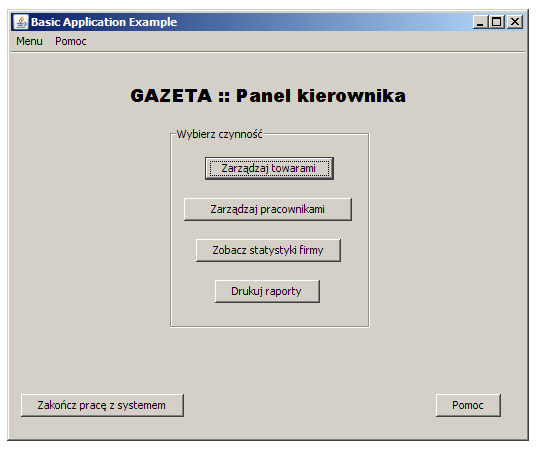
\includegraphics[width=1\textwidth]{gfx/szef_szefow.png}
\caption{Widok panelu kierownika}
\end{figure}
Wybór opcji "Zarządzaj towarami", "Zarządzaj pracownikami" lub "Zobacz statystyki firmy" powoduje otwarcie nowego okna z~odpowiednim panelem.

Wybór opcji "Drukuj raporty" powoduje automatyczne wygenerowanie i~wydrukowanie wszystkich logów systemowych i~raportów od ostatniego drukowania.
\clearpage
\subsubsection{Panel zarządzania towarami}
\begin{figure}[h]
\begin{center}
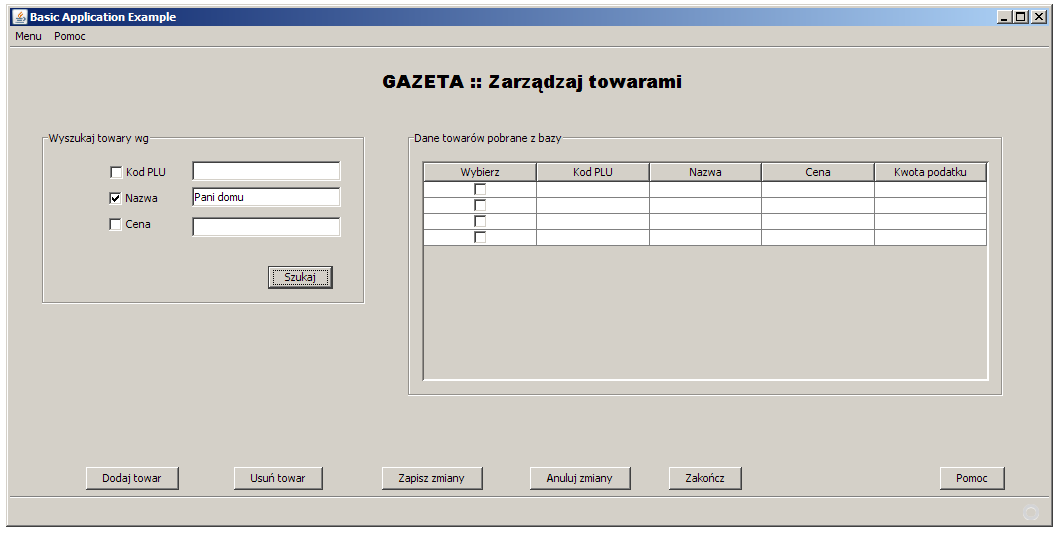
\includegraphics[width=20cm,angle=90,keepaspectratio]{gfx/zarzadzaj_towarami.png}
\end{center}
\caption{Widok panelu zarządzania towarami}
\end{figure}
W~celu znalezienia informacji o towarze w~formularzu po~lewej stronie należy wprowadzić dane dla wyszukiwarki i~zaznaczyć kryteria, według których ma się odbywać wyszukiwanie. W dalszej kolejności, po~wybraniu opcji "Szukaj" w~tabelce po~prawej automatycznie pojawić się pobrane z~bazy dane znalezionych towarów pasujących do~kryteriów wyszukiwania.

W~celu usunięcia towaru znajdującego się w~tabelce z~bazy należy zaznaczyć pole "Wybierz" w~tabelce w~wierszu z~tym towarem, a następnie wybrać opcję "Usuń towar".

W~celu edytowania właściwości towaru znajdującego się w~tabelce należy zaznaczyć pole "Wybierz" w~tabelce w~wierszu z~tym towarem, zmienić zawartość odpowiednich pól w~tym wierszu (np. jeśli chcemy zmienić cenę towaru, wpisać nową wartość w~kolumnie "Cena"), a następnie wybrać opcję "Zapisz zmiany". Można edytować właściwości więcej niż jednego towaru naraz (należy wtedy zaznaczyć pole "Wybierz" przy~każdym edytowanym towarze). Aby~anulować wprowadzone do~tabelki, ale jeszcze nie zapisane zmiany, należy wybrać opcję "Anuluj zmiany".

W~celu dodania towaru do~bazy należy wybrać opcję "Dodaj towar" - w~tabelce pojawi się nowy, pusty wiersz, do~którego należy wprowadzić dane nowego towaru, a następnie zapisać zmiany tak, jak w~przypadku edycji właściwości towaru (poprzez opcję "Zapisz zmiany").

Aby~zamknąć panel zarządzania towarami i~powrócić do~panelu kierownika, należy wybrać opcję "Zakończ".
\clearpage
\subsubsection{Panel zarządzania pracownikami}
\begin{figure}[h]
\begin{center}
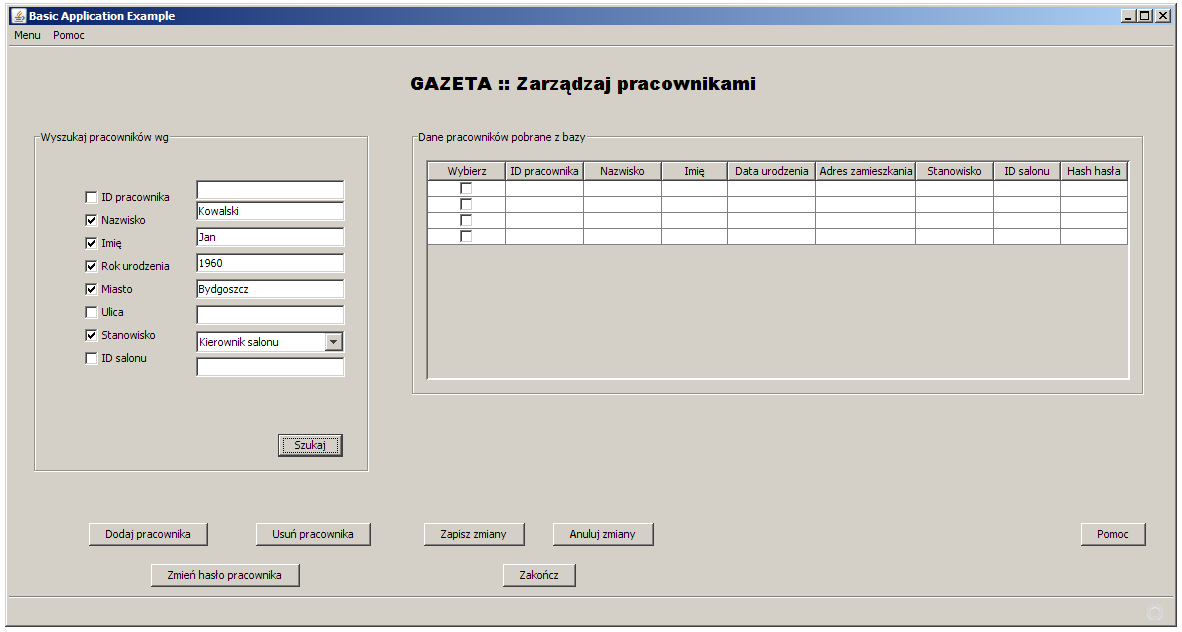
\includegraphics[width=20cm,angle=90,keepaspectratio]{gfx/zarzadzaj_pracownikami.png}
\end{center}
\caption{Widok panelu zarządzania pracownikami}
\end{figure}
W~celu znalezienia informacji o pracowniku w~formularzu po~lewej stronie należy wprowadzić dane dla wyszukiwarki i~zaznaczyć kryteria, według których ma się odbywać wyszukiwanie. W dalszej kolejności, po~wybraniu opcji "Szukaj" w~tabelce po~prawej automatycznie pojawić się pobrane z~bazy dane znalezionych pracowników pasujących do~kryteriów wyszukiwania.

W~celu usunięcia pracownika, którego dane znajdują się w~tabelce, z~bazy należy zaznaczyć pole "Wybierz" w~tabelce w~wierszu z~danymi tego pracownika, a następnie wybrać opcję "Usuń pracownika".

W~celu edytowania danych pracownika znajdujących się w~tabelce należy zaznaczyć pole "Wybierz" w~tabelce w~wierszu z~danymi tego pracownika, zmienić zawartość odpowiednich pól w~tym wierszu (np. jeśli chcemy zmienić ID salonu, wpisać nową wartość w~kolumnie "ID salonu"), a następnie wybrać opcję "Zapisz zmiany". Można edytować dane więcej niż jednego pracownika naraz (należy wtedy zaznaczyć pole "Wybierz" w~każdym wierszu z~edytowanymi danymi pracownika). Aby~anulować wprowadzone do~tabelki, ale jeszcze nie zapisane zmiany, należy wybrać opcję "Anuluj zmiany".

Ponieważ w~bazie przechowywany jest hash hasła, a nie samo hasło, są dwa sposoby zmiany hasła pracownika. Pierwszy to wpisanie edycja hasha w~tabelce (postępując tak, jak przy~zmianie np. nazwiska pracownika). Drugi to zaznaczenie pola "Wybierz" przy~danych wybranego pracownika (lub kilku pracowników, jeśli chcemy ustawić takie samo hasło pewnej grupie pracowników) i~wybór opcji "Zmień hasło pracownika". Po jej wybraniu w~nowym oknie zostanie otwarty panel zmiany hasła.

W~celu dodania nowego pracownika do~bazy należy wybrać opcję "Dodaj pracownika" - w~tabelce pojawi się nowy, pusty wiersz, do~którego należy wprowadzić dane nowego pracownika, a następnie zapisać zmiany tak, jak w~przypadku edycji danych pracownika (poprzez opcję "Zapisz zmiany").

Aby~zamknąć panel zarządzania pracownikami i~powrócić do~panelu kierownika, należy wybrać opcję "Zakończ".
\clearpage
\subsubsection{Panel zmiany hasła}
\begin{figure}[h]
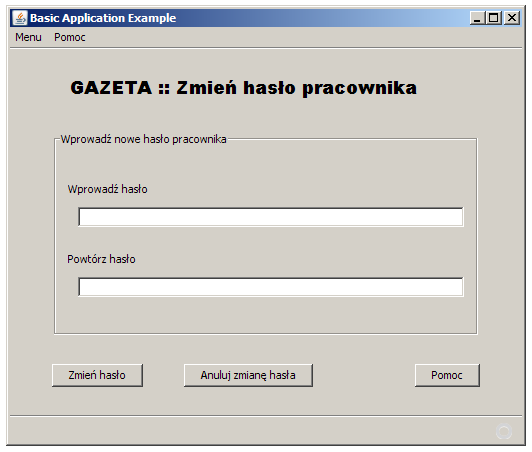
\includegraphics[width=1\textwidth]{gfx/zmiana_hasla.png}
\caption{Widok panelu zmiany hasła}
\end{figure}
W formularzu należy wpisać nowe hasło pracownika i~powtórzyć je.

Aby~zatwierdzić zmianę i~powrócić do~panelu zarządzania pracownikami, należy wybrać opcję "Zmień hasło" (hash hasła zostanie wówczas zapisany w~bazie danych).

Aby~anulować zmianę i~powrócić do~panelu zarządzania pracownikami, należy wybrać opcję "Anuluj zmianę hasła".
\clearpage
\subsubsection{Panel statystyk firmy}
\begin{figure}[h]
\begin{center}
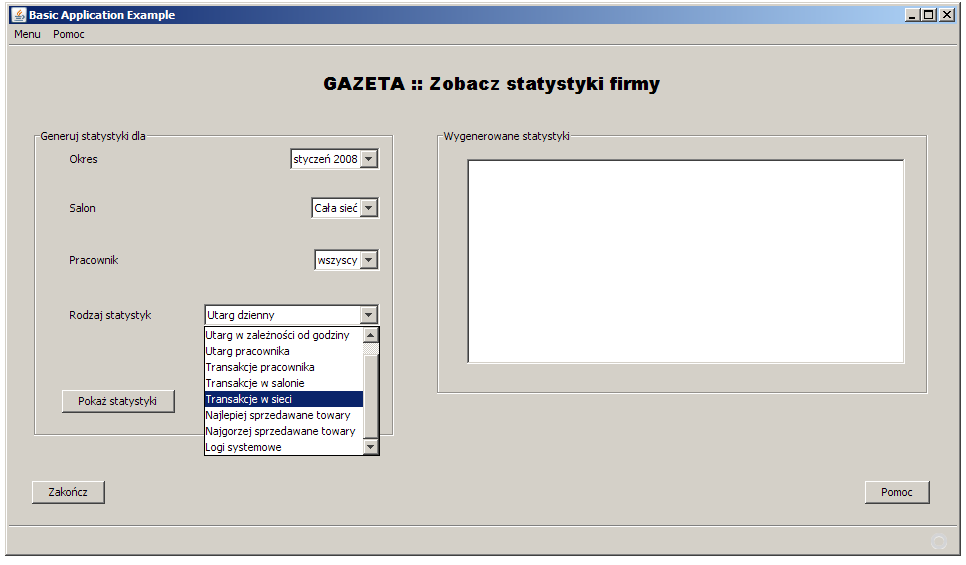
\includegraphics[width=20cm,angle=90,keepaspectratio]{gfx/stat_firmy.png}
\end{center}
\caption{Widok panelu statystyk firmy}
\end{figure}
W formularzu należy wybrać okres, za~który mają został wygenerowane statystyki, pracowników i~salony, których statystyki mają dotyczyć, oraz~rodzaj statystyk. Wybór opcji "Pokaż statystyki" powoduje wygenerowanie (na podstawie danych pobranych w~tym celu z~bazy) statystyk odpowiadających danym z~formularza i~wyświetlenie ich w~formie graficznej (lub tekstowej, w~przypadku logów systemowych) w~ramce "Wygenerowane statystyki".

Aby~zakończyć oglądanie statystyk salonu i~powrócić do~panelu kierownika, należy wybrać opcję "Zakończ".
\clearpage
\subsection{Dodatkowe opcje}
Dodatkowo we wszystkich panelach w~prawym dolnym rogu umieszczony jest przycisk "Pomoc", po~wciśnięciu którego wyświetlana jest pomoc dotycząca bieżącego panelu.